\section{النماذج السابقة للمحول}
صمم نموذج المحول
\textLR{\cite{Vaswani17}}
ليكون إحدى نماذج
\textLR{seq2seq}،
وهي نماذج يكون كل من دخلها وخرجها عبارة عن سلاسل من العناصر. من الممكن أن تكون السلسلة أي نوع من المعلومات ككلمات، صور، محارف أو غيرها
\textLR{\cite{web:visualize}}.
\newline
معظم تطبيقات نماذج
\textLR{seq2seq}
 كانت في مجال معالجة اللغات الطبيعية
\textLR{Natural Language Processing NLP}
 أي يكون الدخل عبارة عن سلسلة من كلمات.
\begin{figure}[h!]
\centerline{
	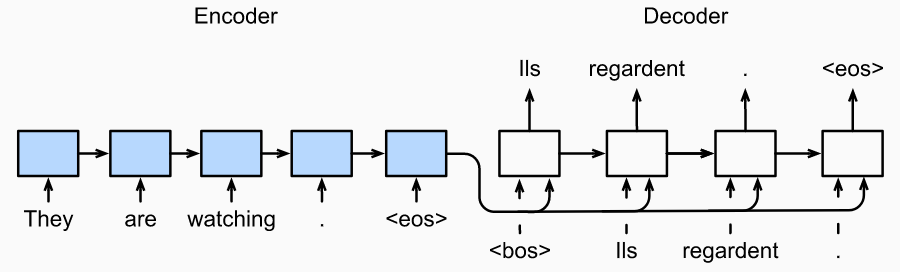
\includegraphics[width=\textwidth]{images/RNN.png}}
\caption{نموذج
\textLR{seq2seq}
مع بنية
\textLR{encoder-decoder}
\textLR{\cite{d2l_rnn}}
}
\label{fig:RNN1}	
\end{figure}
%قبل استخدام نموذج المحول
كانت البنية الأساسية لنماذج
\textLR{seq2seq}
هي الشبكات العصبونية العودية
\textLR{recurrent neural networks RNN}.
ولفهم تطور بنية المحول يجب أن نفهم البنية العامة للشبكات العودية وهو ما سنذكره في الفقرة القادمة.
\newline
\subsection{الشبكات العصبونية العودية
\textLR{RNN}
}
تُستخدم
\textLR{RNN}
 بشكل رئيسي للتعرف على الأنماط في المعطيات التسلسلية، كالنصوص، الفيديوهات أو أي متسلسلة زمنية. وما يميزها
 عن الشبكات العصبونية التقليدية
\textLR{MLP Multilayer perceptron}
 هو كيفية مرور المعلومات من خلالها
\textLR{\cite{RNN-gentleIntro}}.

\begin{figure}[H]
	\centerline{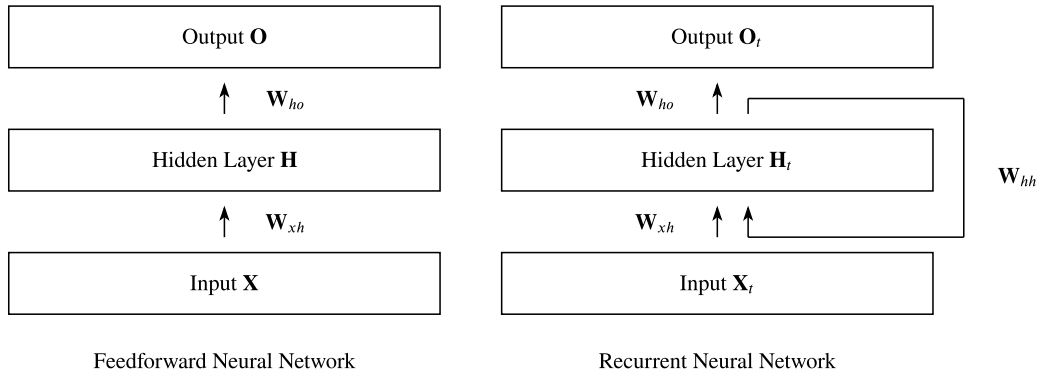
\includegraphics[width=\textwidth]{images/RNN_gentle_introduction.png}}
	\caption{
	\begin{footnotesize}
			الفرق بين مرور المعلومات بين الشبكات العودية - اليمين، والشبكات التقليدية - اليسار
\textLR{\cite{RNN-gentleIntro}}
	\end{footnotesize}
		}
	\label{fig:RNN2}
\end{figure}
يوضح الشكل
\ref{fig:RNN2}
 الاختلاف بين
\textLR{MLP}
 و
\textLR{RNN}،
 حيث تمرر شبكات 
\textLR{MLP}
المعلومات بدون وجود أي حلقات على العكس من شبكات
\textLR{RNN}.
حيث يحسب الخرج في شبكات
\textLR{MLP}
 كما في المعادلات
\ref{eq:mlp}
\begin{equation}
	\begin{split}
	& H = \phi_h (XW_{xh} + b_h)\\
	& O = \phi_o (HW_{ho} + b_o)\\
	\end{split}
	\label{eq:mlp}
\end{equation}
حيث $H$ خرج الطبقة المخفية، 
$\phi_h$
تابع تفعيل الطبقة المخفية،
$O$
الخرج النهائي،
$\phi_o$
تابع تغعيل طبقة الخرج، 
$W,b$
مصفوفات الأوزان وأشعة الانحياز.
\newline
أما في 
\textLR{RNN}
فمعادلة الخرج في كل خطوة زمنية
$t$
تحسب من خلال المعادلات 
\ref{eq:RNN}
\begin{equation}
\begin{split}
	&H_t = \phi_h(X_t W_{xh} + H_{t-1} W_{hh} + b_h)\\
	& O_t = \phi_o (H_t W_{ho} + b_o)\\
\end{split}
\label{eq:RNN}
\end{equation}
حيث
$H_t$
يدعى بالحالة المخفية
\textLR{hidden state}
في اللحظة
$t$.
\newline
نلاحظ أنه في كل خطوة زمنية لحساب الخرج نحتاج إلى الدخل
$X_t$
وإلى الحالة المخفية في الخطوة الزمنية السابقة كما هو موضح في الشكل 
\ref{fig:RNN3}،
والذي يبين مخارج ومداخل
\textLR{RNN}
بعد نشر الشبكة من أجل كل خطوة زمنية.
\begin{figure}[h!]
	\centerline{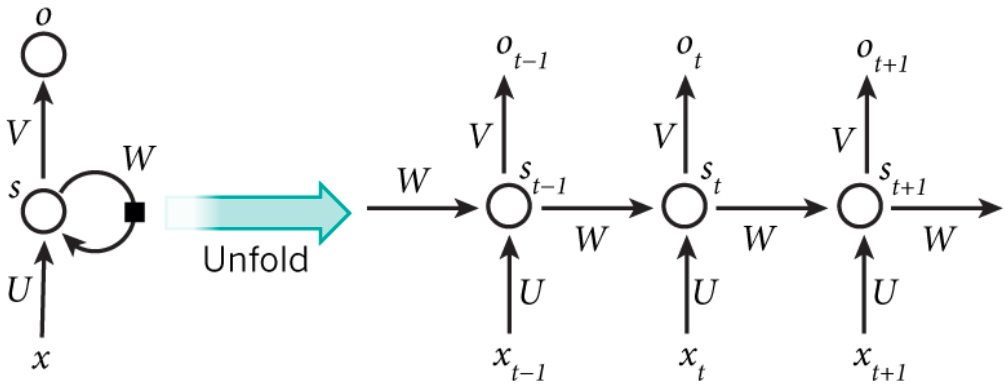
\includegraphics[width=\textwidth]{images/RNN_unfold}}
	\caption{
		نشر الشبكة العصبونية العودية
		\textLR{RNN}
		من أجل عدة لحظات زمنية
		\textLR{\cite{RNN-unfold}}}
	\label{fig:RNN3}
\end{figure}
%نلاحظ أيضا أنه لحساب الخرج في لحظة زمنية
%$t$
%نحتاج إلى دخل السلسلة في هذه اللحظة
%$X_t$
%وإلى الحالة المخفية في اللحظة السابقة
%$H_{t-1}$
%أو
%$s_{t-1}$
%كما هو موضح في الشكل
%\ref{fig:RNN3}
%والمعادلات
%\ref{eq:RNN}.
\newline
\subsubsection{مشكلات 
\textLR{RNN}}
إحدى سلبيات شبكات
\textLR{RNN}
 هي معالجة العناصر بشكل تسلسلي، فكما رأينا في الفقرة السابقة فإن الخرج في كل خطوة زمنية يحتاج إلى معالجة المداخل السابقة بشكل تسلسلي و هذا مايجعل زمن التدريب طويلاً، وبسبب بنية الشبكة تصبح المعالجة بشكل تفرعي أمراً صعباً أو حتى مستحيل
\textLR{\cite{TransformerCV}}.
المشكلة الثانية هي تلاشي المشتقات
\textLR{vanishing gradient}
وهو ما يزيد من صعوبة التدريب وبخاصة في حالة السلاسل الطويلة، إحدى أشهر الحلول لتقليل أثر هذه المشكلة هي باستخدام
\textLR{Long Short-Term Memory LSTM}.
من الممكن أن تختلف أبعاد سلسلتي الدخل والخرج ولحل هذا الاختلاف في الطول يمكن استخدام شبكتين عوديتين منفصلتين الأولى نسميها الـ
\textLR{encoder}
المرمز والثانية الـ
\textLR{decoder}
مفكك ترميز.
\subsection{
بنية المرمز ومفكك الترميز
}
يعالج المرمز كل عنصر من عناصر سلسلة الدخل ويستخرج المعلومات ويضعها في شعاع يسمى شعاع السياق
\textLR{context vector}،
بعد انتهاء المرمز من معالجة كامل عناصر الدخل يرسل شعاع السياق إلى مفكك الترميز
%\textLR{decoder}
 ليقوم بتوليد سلسلة الخرج بشكل تتابعي كما في الشكل
\ref{fig:RNN1}.
\newline
المشكلة الأساسية في هذه النماذج هي كيفية توليد شعاع السياق ليعبر بأفضل طريقة ممكنة عن معلومات سلسلة الدخل. فإذا كان شعاع السياق هو الحالة المخفية لآخر خطوة زمنية في سلسلة الدخل عندها لن يعبر بشكل فعال عن بدايات السلسلة وخصوصاً في حالة سلسلة الدخل الطويلة
\textLR{\cite{IllustratedAttention}}.
عندها يمكن أن يكون شعاع السياق عبارة عن كامل الحالات المخفية لكل خطوة زمنية في سلسلة الدخل، أو أن ينتج عن تعديل هذه الحالات المخفية بتطبيق تابع معين، ومن هنا ظهرت فكرة الانتباه 
\textLR{attention}،
وذلك بالتركيز فقط على الأجزاء المهمة وجعل الأجزاء غير المهمة أقل تأثيراً
\textLR{\cite{TransformerCV}}.
بما أن المشكلة الأساسية هي كيفية توليد شعاع السياق كان هناك الكثير من الأبحاث لتحسين تمثيل هذا الشعاع من أبرزها
\textLR{\cite{Bahdanau2016},\cite{Luong2015}}.
إذ كانت هذه الأعمال بدايات فكرة الانتباه، والذي أظهر نتائج جيدة ومبشرة في تطبيقات ترجمة الآلة، وخاصة في حالة الأبعاد الكبيرة لسلاسل الدخل
\textLR{\cite{IllustratedAttention}}.

\section{المحول \label{section:transformer}}
ظهر نموذج المحول
\textLR{Transformer\cite{Vaswani17}}
في عام $2017$ ولأول مرة تم اختبار نموذج يعتمد بشكل كامل على توابع الانتباه ويستغني عن
\textLR{RNN}،
 مما جنب نموذج المحول العديد من مشاكل هذا النوع من الشبكات والتي أهمها عدم القدرة على المعالجة التفرعية لعناصر الدخل، إذ أن أحد ميزات المحول هي قابلية معالجة العمليات الحسابية بشكل تفرعي كما سنرى لاحقاً وهذا ما يسرع عملية التدريب و الـ 
\textLR{inference}
في حال وجود
\textLR{GPU}.
\subsection{بنية المحول}
\begin{table}[h!]
	\centering
	\begin{tabular}{c c} 
		\hline
		\textLR{sympol} & \textLR{meaning} \\ [0.5ex] 
		\hline\hline
		$d$ & \textRL{بعد النموذج}  \\ 
		$h$ &  \textLR{MHA} \textRL{عدد الرؤوس في}\\
		$L$ & \textLR{tokens} \textRL{عدد عناصر سلسلة الدخل، أو عدد الـ}\\
		$X \in \mathds{R}^{L \mathsf{x}d}$&\textRL{دخل المرمز}\\
		$W^k \in \mathds{R}^{d \mathsf{x} d_x}$&\textLR{key}\textRL{مصفوفة الأوزان لشعاع الـ }\\
		$W^q \in \mathds{R}^{d \mathsf{x} d_x}$&\textLR{query}\textRL{مصفوفة الأوزان لشعاع الـ }\\
		$W^v \in \mathds{R}^{d \mathsf{x} d_v}$&\textLR{value}\textRL{مصفوفة الأوزان لشعاع الـ }\\
		$W^k_i,W^q_i \in \mathds{R}^{d\mathsf{x}d_k/h};W^v_i\in \mathds{R}^{d\mathsf{x}d_v/h}$&\textRL{مصفوفات الأوزان لكل  رأس}\\
		$W^o \in \mathds{R}^{d_v \mathsf{x}d}$&\textRL{مصفوفة الأوزان لشعاع الخرج }\\
		$Q = XW^q \mathds{R}^{L \mathsf{x}d_k}$&\textLR{query}\\
		$K = XW^k \mathds{R}^{L \mathsf{x}d_k}$&\textLR{key}\\
		$V = XW^v \mathds{R}^{L \mathsf{x}d_v}$&\textLR{value}\\
		\hline
	\end{tabular}
	\caption{\textRL{الرموز المستخدمة في شرح بنية المحول مع أبعاد المصفوفات}}
	\label{table:transformer_sympols}
\end{table}          
إن التطبيق الأساسي لنموذج المحول الأصلي
\textLR{\cite{Vaswani17}}
هو ترجمة الجمل من اللغة الإنكليزية إلى لغات أخرى، إذ أن دخل النموذج سلسلة من الكلمات (عدة جمل)، كل كلمة يتم التعبير عنها بشعاع من الأرقام ندعوه بالـ
\textLR{token}،
فيكون دخل المرمز هو عبارة عن مصفوفة أشعة
$X \in \mathds{R}^{L \mathsf{x}d}$.
\newline
لتمييز مكان كل عنصر من السلسلة  يتم إضافة قيم للترميز المكاني
\textLR{positional encoding PE}.
خرج كل طبقة من طبقات المرمز وطبقات مفكك الترميز
هو مصفوفة أشعة بأبعاد
$L \mathsf{x} d$.
كما يوضح الشكل
\ref{fig:Transformer}
يتكون كل من المرمز و مفكك الترميز
 من عدة كتل متسلسلة ومتطابقة في البنية.
\subsection{المرمز}
بداخل كل كتلة مرمز كتلتان أساسيتان كما في الشكل
\ref{fig:enc_dec}
 الأولى لحساب الانتباه الذاتي متعدد الرؤوس 
\textLR{Multi-Head Self Attention MHA},
مهمة هذا التابع هو تعديل تمثيل عناصر سلسلة الدخل بحسب السياق.
والكتلة الثانية هي شبكة عصبونية
\textLR{FFN}
تتكون من طبقتين مع تابع تفعيل 
\textLR{ReLU}
بحسب المعادلة
\ref{eq:MLP}.
\begin{equation}
FFN(x) = max(0,xW_1+b_1)W_2+b_2
\label{eq:MLP}
\end{equation}
تطبق هذه الشبكة على كل
\textLR{token}
أو عنصر دخل بشكل منفصل ومتطابق، وهذا مانسميه
\textLR{position-wise}
كما في الشكل
\ref{fig:positionWise}،
مما يجعل المحول قادر على إجراء الحسابات بشكل تفرعي.
من أجل كل من الكتلتين السابقتين يتم تطبيق
\textLR{residual connection \cite{residual}}،
 متبوعة بـ
\textLR{layer normalization\cite{LN}}.
\newline
%$\text{\textLR{LayerNorm}}(x+\text{\textLR{Sublayer}}(x))$
%حيث
%\textLR{sublayer}
%هي تابع الانتباه أو الشبكة العصبونية الأمامية.
\begin{figure}[H]
	\centerline{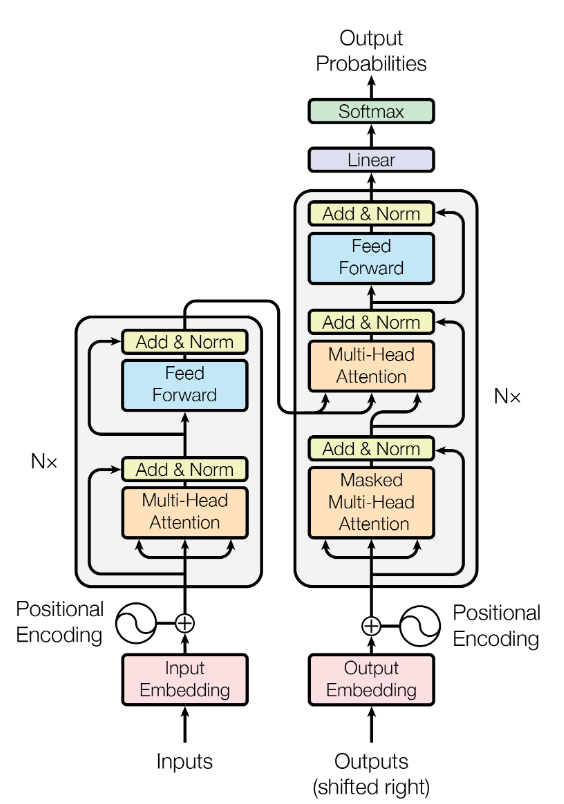
\includegraphics[scale=0.5]{images/Transformer}}
	\caption{\textRL{البنية الأساسية للمحول}
	\textLR{\cite{Vaswani17}}}
	\label{fig:Transformer}
\end{figure}

\begin{figure}[h!]
	\centerline{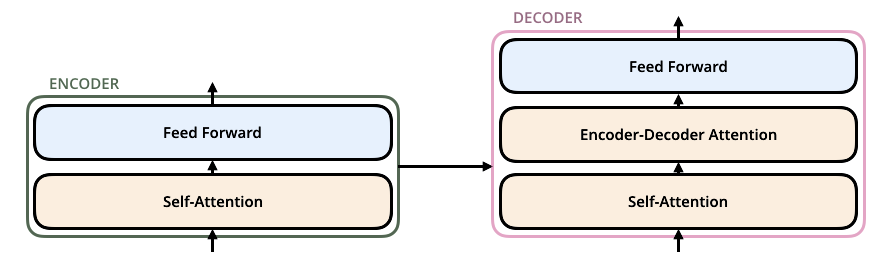
\includegraphics[scale=0.3]{images/encoder_decoder_illustrated_transformer}}
	\caption{البنية الأساسية للمرمز و مفكك الترميز
		داخل المحول
		\textLR{\cite{illustratedTransformer}}}
	\label{fig:enc_dec}
\end{figure}

\begin{figure}[h!]
	\centerline{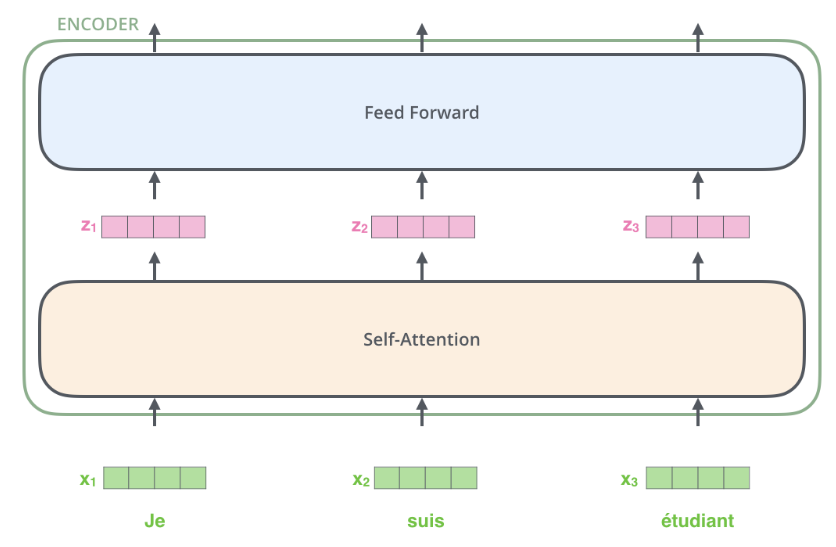
\includegraphics[scale=0.3]{images/position_wise_illustrated_transformer}}
	\caption{\textRL{تطبيق التوابع داخل المحول لكل عنصر دخل بشكل تفرعي}
	\textLR{\cite{illustratedTransformer}}}
	\label{fig:positionWise}
\end{figure}
 
\subsection{مفكك الترميز}
يوضح الشكلان
\ref{fig:Transformer}،\ref{fig:enc_dec}
بنية مفكك الترميز،
وكما في المرمز فإنه يتكون بالإضافة إلى كتلتي الانتباه الذاتي والشبكة الأمامية فإنه أيضاً يحتوي على كتلة إضافية وهي الانتباه التقاطعي متعدد الرؤوس.
%\ref{MCHA}
%دخل هذا التابع هو دخل مفكك الترميز بعد إضافة الترميز المكاني، بحيث يكون %دخل مفكك الترميز  هو خرج آخر طبقة في المرمز.
في خوارزمية المحول الأساسية
\textLR{\cite{Vaswani17}}
يكون دخل مفكك الترميز  هو خرج آخر طبقة في المرمز.
\subsection{ترميز المعلومات المكانية
\textLR{positional encoding\label{PE}}}
كما ذكرنا سابقاً فإن معظم نماذج
\textLR{seq2seq}
قبل ظهور نموذج المحول
\textLR{\cite{Vaswani17}}
كانت تستخدم الشبكات العودية
\textLR{RNN}
مع 
\textLR{LSTM}،
وهذا النوع من الشبكات يحافظ على المعلومات المكانية النسبية لعناصر سلسلة الدخل،  لكن الاستغناء عن شبكات 
\textLR{RNN}
والاستعانة فقط بتوابع الانتباه لمعالجة السلاسل يفقد المعلومات المكانية.
\newline
لمعالجة هذه المشكلة كان من اللازم إدخال المعلومات المكانية للسلسلة بشكل ما، هنا تم طرح طريقة ترميز الموقع لإضافة المعلومات المكانية لكل عنصر من عناصر السلسلة وذلك بإضافة قيم مستخرجة من توابع بترددات مختلفة كما في المعادلات 
\ref{eq:PE}
\textLR{\cite{Vaswani17}}.
\begin{equation}
\begin{split}
	&PE_{(pos,2i)} = sin(pos/1000^{2i/d_{model}})\\
	&PE_{(pos,2i+1)} = cos(pos/1000^{2i/d_{model}})\\
\end{split}
\label{eq:PE}
\end{equation}
حيث 
\textLR{pos}
موقع عنصر الدخل من السلسلة، و
$i$
هو البعد 
\textLR{dimension}.
ويتم إضافة قيم هذه التوابع إلى دخل كل من المرمز ومفكك الترميز.
\newline
اختبرت العديد من الأبحاث طرق الترميز المكاني، فأبسط الأشكال هي إسناد رقم طبيعي أو حقيقي مميز أو عدد ضمن المجال
$[0,1]$
 إلى كل عنصر من عناصر السلسلة
\textLR{\cite{web:PE}}.
\newline
لكن هذه الطرق البسيطة لم تحسن النتائج لأنها لم تستطع أن تجعل النموذج يلتقط معلومات المواقع بين العناصر.
هنا اقترح البحث 
\textLR{\cite{Vaswani17}}
أن يكون ترميز الموقع تابع جيبي كما في المعادلات 
\ref{eq:PE}،
إذ يمكن اعتبار  سلسلة الدخل سلسلة زمنية وكل عنصر هو خرج السلسلة عند خطوة زمنية معينة
\textLR{\cite{web:PE}}،
هذه الطريقة في التفكير ساعدت النموذج على كشف معلومات الموقع النسبية بين العناصر.
 
في الملاحق المستخدم في بحثنا
\textLR{SwinTrack\cite{swinTrack}\ref{section:swintrack}}
تم استخدام 
\textLR{untied PE \cite{untiedPE}}
مع بارامترات قابلة للتدريب.